\chapter{Policy Implementation and Evaluation in an IFC-enabled Browser}
\label{ch:eval}
\blfootnote{The content of this
  chapter is based partly on the work published as part of the paper,
  ``WebPol: Fine-grained Information Flow Policies for Web Browsers''~\cite{webpol}} 

This chapter describes the implementation of \sys~(Chapter~\ref{ch:webpol}) 
and the LIR policy (Chapter~\ref{ch:lir}) on top of
an existing IFC-instrumentation~\cite{just11PLASTIC,post14,csf15} 
(referred to as WebIFC in the remaining of this chapter). 
WebIFC targets WebKit, the browser engine used 
in Safari, for enforcing 
dynamic IFC in the three main components of the engine --- JavaScript 
bytecode interpreter, the document object model (DOM) engine, and the
event handling mechanism. 

Labels in WebIFC are word size bit-sets (currently 64 
bits); each bit in the bit-set represents label from a distinct domain
(like google.com). Join on labels is simply bitwise or. 
WebIFC adds labels to all data structures, including
registers, objects, object properties and scope chain pointers, and  
attach security labels to every node in the DOM graph and all its 
properties, including pointer to other nodes. 
In WebIFC, the code is instrumented to propagate explicit and 
implicit labels and implement the permissive-upgrade check. 
Specifically, WebKit’s JavaScript bytecode interpreter 
(JavaScriptCore) for enforcing dynamic IFC for 
JavaScript~\cite{just11PLASTIC,post14}. In WebKit, bytecode is generated
by a source-code compiler and organized into code blocks. Each code
block is a sequence of bytecodes with line numbers and corresponds to
the instructions for a function or an \texttt{eval} statement. A code
block is generated when a function is created or an \texttt{eval} is
executed. WebIFC performs control flow analysis on a
code block when it is created and generates a CFG for it before it
starts executing. The IPDs of its nodes are calculated by static
analysis of its bytecode; they are computed using an algorithm by
Lengauer and Tarjan with CFG as an input to the
algorithm~\cite{Lengauer}. The formalization of the bytecodes, the
semantics of its bytecode interpreter with the instrumentation of
dynamic IFC, and the proof of correctness of instrumentation of the
bytecodes with the IFC semantics is shown in~\cite{post14Extended}.
Additionally, all native JavaScript methods in the Array, RegExp, 
and String objects are instrumented in WebIFC and appropriate  
IFC checks in the native C code implementing all DOM APIs up
to Level 3 are added~\cite{csf15}. 
WebIFC also modifies the event handling loop, labeling every event and
event handler based on their formalization of the event handling loop
with the IFC checks~\cite{csf15}.  

WebIFC enforces termination-insensitive non-interference in all 
the major components of WebKit while tracking labels 
at a fine-granularity. This thesis adds additional instrumentation 
on top of WebIFC for enforcing the ideas presented 
earlier. For exceptions, a synthetic exit node is added to the CFG
along with the edges as described earlier in
Section~\ref{sec:excsen}. Additional changes are required to the
compiler to make it compliant with the instrumentation. The
modification is to emit a slightly different, but functionally
equivalent bytecode sequence for \texttt{finally} blocks; 
this is needed for accurate computation of IPDs. 


\section{Implementation and Evaluation of \sys}
\label{sec:implpol}
\subsection{Implementation of \sys}
{\sys} is prototyped in WebKit on top of WebIFC. To implement
{\sys}, the HTML parser was modified to distinguish policy files
(extension \texttt{.policy}) from other JavaScript files and to give
policy code extra privileges. Two new JavaScript API functions ---
\texttt{setLabel()} and \texttt{setContext()} --- were added. Finally,
the event dispatch logic was modified to trigger policy handlers
before other handlers. In all, 25 lines in the code of the parser were
modified, 60 lines for the two new API functions were added and 110
lines in the event dispatch logic were modified. Thus, implementing
{\sys} has low overhead, and can be ported to other browsers easily.

\subsection{Evaluation of \sys}
\label{sec:eval-webpol}
The goal of the evaluation is two-fold. The first goal is to measure
the overhead of the system with IFC enforcement and {\sys}, both in
parsing and installing policies during page load and for executing
policy handlers later. This is done by running a few benchmarks, by measuring the
overhead for the examples presented in Section~\ref{sec:examples}, and
for two real-world websites. Second, to 
understand whether {\sys} can be used easily, {\sys} policies are
applied to two real-world websites. All the experiments were
performed on a 3.2GHz Quad-core Intel Xeon processor with 8GB RAM,
running Mac OS X version 10.7.4 using Safari 6.0. The implementation
and evaluation is done on WebKit nightly build $\#r122160$. As 
WebIFC does not cover JIT, JIT support was
disabled in all the experiments. 

\subsubsection{Performance Overheads on Synthetic Examples}
To measure the instrumentation's runtime overhead, four examples from 
Chapter~\ref{sec:examples} (Examples~1,~2 and the two sub-examples of
Example~3) were tested in three different configurations:
\textbf{Base}---uninst\-ru\-mented browser, no enforcement;
\textbf{WebIFC}---existing instrumented browser with IFC checks, but no
policy handlers (everything is labeled public);
\textbf{{\sys}}---instrumented browser running policy handlers.

\newcolumntype{C}[1]{>{\centering\let\newline\\\arraybackslash\hspace{0pt}}m{#1}}

\begin{table}[tbp]
\centering
\begin{tabular}{ | C{2cm} || C{1.5cm} | C{1.5cm} | C{1.5cm} || C{1.5cm} | C{1.5cm} | C{1.5cm} |}
\hline
\multicolumn{1}{|c||}{ } &
\multicolumn{3}{ c ||}{JavaScript Execution Time} &
\multicolumn{3}{ c |}{Page Load Time} \\
\hline
 Example \# & \textbf{Base} & \textbf{WebIFC} & \textbf{\sys} & \textbf{Base} & \textbf{WebIFC} & \textbf{\sys} \\
  \hhline{|=#=|=|=#=|=|=|} 
  Example~1 & 2430 & 2918 (+20.1\%) & 2989 (+1.9\%) & 16 & 17 (+6.3\%) & 19 (+12.5\%) \\  
\hline
  Example~2 & 3443 & 4361 (+26.7\%) & 5368 (+29.2\%) & 41 & 43 (+4.9\%) & 46 (+7.2\%)\\ 
\hline
  Example~3 (count) & 1504 & 1737 (+15.5\%) & 1911 (+11.6\%) & 24 & 25 (+4.2\%) & 31 (+25.0\%) \\
\hline
  Example~3 (presence) & 1780 & 2095 (+17.7\%) & 2414 (+18.9\%) & 26 & 28 (+7.7\%) & 30 (+7.7\%)\\
\hline
\end{tabular}
\caption{Performance of examples from Section~\ref{sec:examples}. All
  time in ms. The numbers in parenthesis are additional overheads
  relative to \textbf{Base}.}
\label{table:eap}
\end{table}

\noindent
\textbf{JavaScript execution time:} The overheads of executing policy
handler code were measured by interacting with all four programs
manually by entering relevant data and performing clicks a fixed
number of times. For each of these configurations, the total time
spent \emph{only in executing JavaScript} was measured, including 
scripts and policies loaded initially with the page and the scripts
and policies executed in response to events. The difference between
\textbf{WebIFC} and \textbf{Base} run times is the overhead of dynamic
IFC, while the difference between the \textbf{\sys} and
\textbf{WebIFC} run times is the overhead of evaluating policy
handlers. Since only JavaScript execution time is measured and
there are no time-triggered handlers in these examples, variability in
the inter-event gap introduced by the human actor does not affect the
measurements.

The left half of Table~\ref{table:eap} shows these observations.
%
All numbers are averages of 5 runs and the standard deviations are
all below 7\%. %\TODO{Fill these numbers}
%
\textbf{WebIFC} adds overheads ranging from 15.5\% to
26.7\% over \textbf{Base}. To this, the policy handlers (\textbf{\sys})
add overheads ranging from 1.9\% to 29.2\%. The \textbf{\sys}
overheads are already modest, but this is also a very challenging
(conservative) experiment for {\sys}. The scripts in 
both sub-examples of Example~3 do almost nothing. The scripts in
Examples~1 and Example~2 are slightly longer, but are still much
simpler than real scripts. On real and longer scripts, the relative
overheads of evaluating the policy handlers is significantly lower as
shown later. Moreover, the baseline in this experiment does not
include other browser costs, such as the cost of page parsing and
rendering, and network delays. Compared to those, both \textbf{WebIFC}
and \textbf{\sys} overheads are negligible.

\noindent
\textbf{Page load time:} The time taken for loading the initial page
(up to the DOMContentLoaded event) was measured separately. The
difference between \textbf{\sys} and \textbf{WebIFC} is the overhead for
parsing and loading policies. The right half of Table~\ref{table:eap}
shows these observations. All numbers are the average of 20 runs and
standard deviations were below 8\%.
{\sys} overheads due to policy parsing and loading range from 7.2\% to
25\% (last column). When the overheads due to taint tracking
(column \textbf{WebIFC}) are added, the numbers increase to 12.1\% to
29.2\%. Note that page-load overheads are incurred only once on every
page (re-)load. 

\subsubsection{Policies on Real-world Websites.}
\label{sec:realpolicies}

Further, {\sys} was evaluated by writing policies for two real-world
applications---a website that deploys a password-strength checker
(similar to Example~1) and a bank log-in page that includes third-party
analytics scripts (similar to Example~3).
The {\sys} policies specified for the password strength checking
website and the bank website with an analytics script are shown in
Listings~\ref{realpolicy1} and~\ref{realpolicy2}, respectively. The
code on lines~\ref{ex:start}--\ref{ex:end} of
Listing~\ref{realpolicy1} allows the strength-checking script to write
back the visual indicator of password strength to the host page's DOM.

\begin{lstlisting}[float, caption=Policy code for password strength
  checking website,label=realpolicy1,language=C,escapechar=\%]
document.getElementById("passwordPwd").setLabel("secret");
document.getElementById("passwordTxt").setLabel("secret");
var x = document.getElementsByTagName("div"); %\label{ex:start}%
var i = 0;
for (i = 0; i < x.length; i++) 
    x[i].setLabel("secret"); %\label{ex:end}%
\end{lstlisting}

\begin{lstlisting}[float, caption=Policy code for bank log-in
  website with an analytics script,label=realpolicy2,language=C] 
var x = document.getElementsByClassName("user"); // username
var y = document.getElementsByClassName("pwd"); // password
for (i = 0; i < x.length; i++) {
    x[i].addEventListener("keypress", function(event){
    event.setLabel("HOST");
    });}
for (i = 0; i < y.length; i++) {
    y[i].addEventListener("keypress", function(event){
    event.setLabel("HOST");
    });}
\end{lstlisting}

\noindent
\textbf{Experience writing policies:} In both cases, meaningful
policies could be specified easily after understanding the code,
suggesting that {\sys} policies can be (and should be) written by
website developers. The policy for the password-strength
checker is similar to Listing~\ref{egscript1} and prevents the
password from being leaked to third-parties. Additional policy code of
4 lines was needed to allow the script to write the results of
the password strength check (which depends on the password) into the
host page.
%
The analytics script on the bank website communicates all
user-behavior to its server.  The policy specified disallows
exfiltration of keypresses on the username and the password text-boxes 
to third-parties.

\begin{table}[tbp]
\centering
\begin{tabular}{ | C{2cm} || C{1.5cm} | C{1.5cm} | C{1.5cm} || C{1.5cm} | C{1.5cm} | C{1.5cm} |}
\hline
\multicolumn{1}{|c||}{ } &
\multicolumn{3}{ c ||}{JavaScript Execution Time} &
                                                       \multicolumn{3}{
                                                         c |}{Page Load Time} \\
\hline
 \multicolumn{1}{|c||}{Website} & \textbf{Base} & \textbf{WebIFC} & \textbf{\sys} & \textbf{Base} & \textbf{WebIFC} & \textbf{\sys} \\
\hhline{|=#=|=|=#=|=|=|} 
 \multicolumn{1}{|c||}{Password} & 79.5 & 115.5 (+45.3\%) & 126 (+13.2\%) & 303 & 429 (+41.6\%) & 441 (+4.0\%)\\  
\hline
 \multicolumn{1}{|c||}{Analytics} & 273.4 & 375.1 (+37.2\%) & 386.1 (+4.0\%) & 2151 & 2422 (+12.6\%) & 2499 (+3.6\%) \\ 
\hline
\end{tabular}
\caption{Performance on two real-world websites. All time in ms. The
  numbers in parenthesis are additional overheads relative to
  \textbf{Base}.}
\label{table:rap}
\end{table}

\noindent
\textbf{Performance overheads:} The performance overheads 
on the two websites were also measured, in the same configurations as
for the synthetic examples. Table~\ref{table:rap} shows the
results. On real-world websites, where actual computation is long, the
overheads of {\sys} are rather small. The overheads of executing
policy handlers, even relative only to \textbf{Base}'s JavaScript
execution time, are 4.0\% and 13.2\%, while the overheads of parsing
and loading policies are no more than 4.0\%. Even the total overhead
of \textbf{WebIFC} and \textbf{\sys} does not adversely affect the user
experience in any significant way.

\section{Implementation and Evaluation of LIR}
\label{sec:impllir}

To implement the LIR semantics described in Chapter~\ref{ch:lir}, the
security label attached to the JavaScript objects and the DOM nodes
was modified to carry a \emph{provenance-label}, representing the dependency
set. The provenance-label is basically a bitvector where each bit
represents a distinct JavaScript object or DOM node. Each bit in the
provenance-label is mapped to a budget, a budget label and an actual
label of the object. The \texttt{setLabel()} API is extended to
include the budget, and the budget label for a JavaScript object or a
DOM node. If the budget is not specified, it is assumed to be
$0$. Similarly, if a budget label is not specified, it is assumed to
be $\bot$. The checks are performed as per the semantics at every
comparison operation assuming an implicit declassification at 
each comparison operation.

\begin{figure}
  \centering
    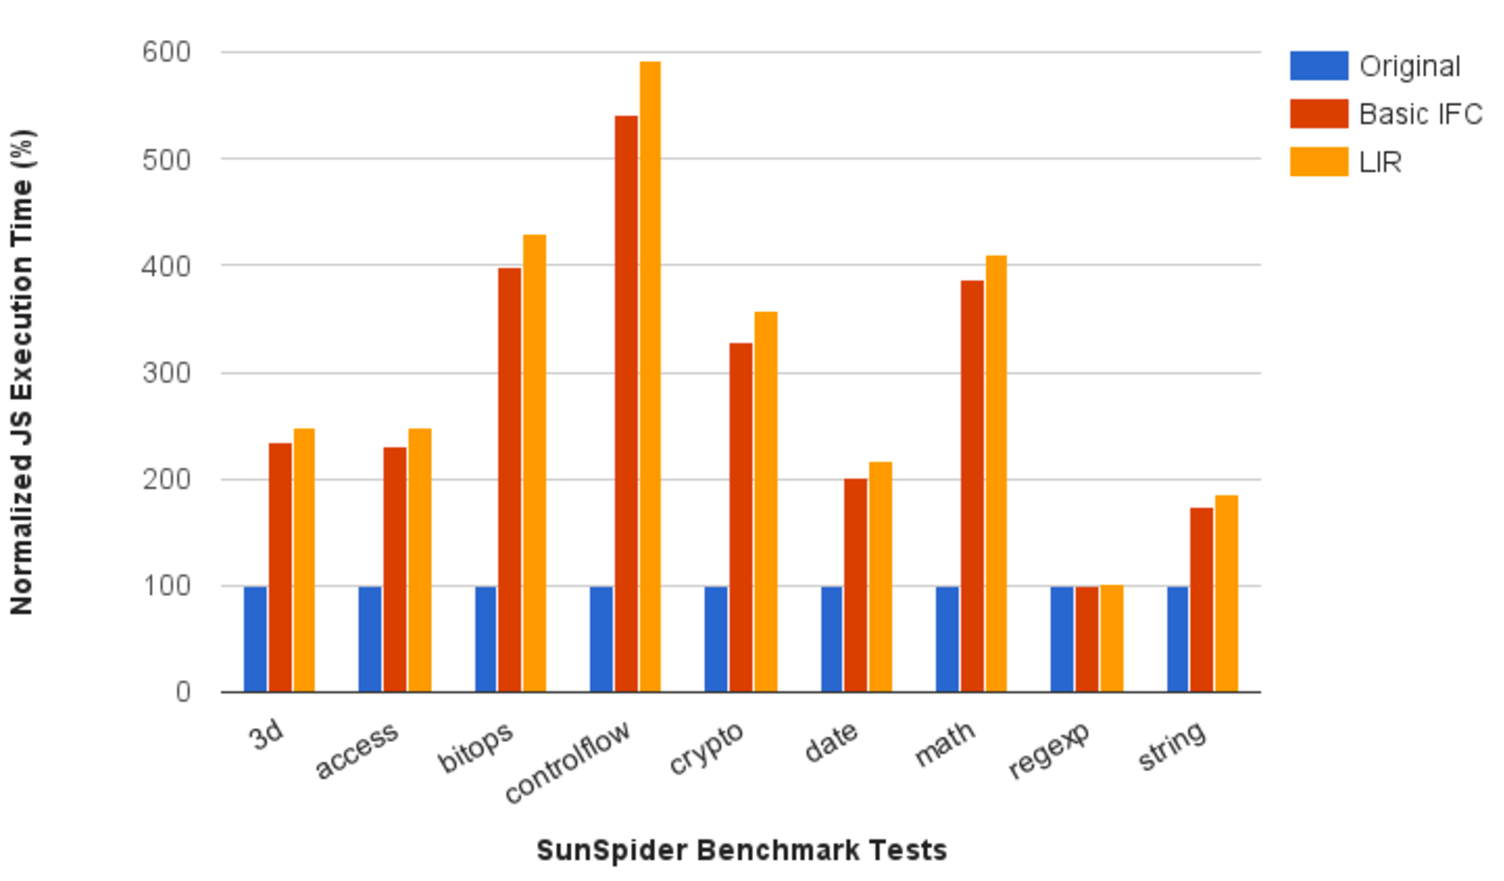
\includegraphics[width=0.8\linewidth]{chapters/browser/LIR.pdf}
  \caption{Overheads of LIR on SunSpider Benchmark Tests}
  \label{fig:dom}
\end{figure}

The performance overhead added as part of the LIR instrumentation in
the IFC-enabled browser is evaluated and compared against the
uninstrumented browser and WebIFC (Basic IFC). 
The performance evaluation was done for the standard
SunSpider 1.0.2 JavaScript benchmark suite on the uninstrumented
browser, on the IFC-instrumented browser and on the LIR instrumented
browser. The average overhead for LIR instrumentation over the
original uninstrumented browser is 170\% and adds only 17\% to the
overhead of \sys.
